\documentclass[10pt]{article}

\usepackage[spanish]{babel} % Idioma del CV en español.
\usepackage[utf8]{inputenc} % Para caracteres especiales. 

\usepackage[a4paper]{geometry} % Definimos estilos de página.
\geometry{top=0.5cm, bottom=0.5cm, left=0.5cm, right=0.5cm} % Eliminamos todos los márgenes posibles.

%----------------------------------------------------------------------------------------------- 
% TEXTO E ICONOS
%-----------------------------------------------------------------------------------------------

\setlength{\parindent}{0mm} % Determinas la sangría en cero.

\usepackage{fetamont} % Fuente.
\usepackage[T1]{fontenc} % Si no usamos este paquete::
                            % * Las palabras que contienen caracteres acentuados no se pueden separar automáticamente,
                            % * No se puede copiar y pegar correctamente tales palabras de la salida (DVI/PS/PDF),
                            % * Y caracteres como el signo de barra vertical, el signo menor que y el signo mayor dan resultados inesperados en el texto.
\usepackage{moresize} % Más tamaños de fuentes.

\usepackage{ragged2e} % Alineación del texto.
\usepackage{fontawesome} % Set de iconos.
\usepackage{paracol} % Para mostrar dos columnas rompibles.

\usepackage{fancyhdr} % Nos proporciona amplias funciones, tanto para construir encabezados y pies de página, como para controlar su uso (por ejemplo, en momentos en que LATEX cambiaría automáticamente el estilo de encabezado en uso).
\pagestyle{empty} % Este comando produce cabeceras y pies de paginas vacíos - sin números de página.

%----------------------------------------------------------------------------------------------- 
% COLOR Y TRANSPARENCIAS
%-----------------------------------------------------------------------------------------------

\usepackage{transparent} % Cómo se puede usar una pila de colores separada para la transparencia, una propiedad además del color.

\usepackage{xcolor} %Ponemos un poco de color, si usamos solo \usepackage{color} tendremos un problema de compatibilidad con el paquete paracol.

\definecolor{maincol}{RGB}{ 225, 0, 0 }
\definecolor{accentcol}{RGB}{ 250, 150, 10 }
\definecolor{darkcol}{RGB}{ 70, 70, 70 }
\definecolor{white}{RGB}{255,255,255} 
\definecolor{darkgray}{HTML}{333333} 
\definecolor{gray}{HTML}{4D4D4D}
\definecolor{sidecolor}{HTML}{E7E7E7}
\definecolor{lightgray}{HTML}{999999}
\definecolor{green}{HTML}{C2E15F}
\definecolor{orange}{HTML}{FDA333}
\definecolor{purple}{HTML}{D3A4F9}
\definecolor{red}{HTML}{FB0B00}
\definecolor{blue}{HTML}{6CE0F1}
\definecolor{mainblue}{HTML}{0E5484}
\definecolor{cerulean}{HTML}{007BA7}
\definecolor{maingray}{HTML}{B9B9B9}
\definecolor{maindarkgray}{HTML}{B3B3B3}

%----------------------------------------------------------------------------------------------- 
%   VARIOS
%----------------------------------------------------------------------------------------------- 

\usepackage[hidelinks]{hyperref} % Para usar links.

\usepackage{tikz} % Para usar gráficos.
\usetikzlibrary{shapes, backgrounds,mindmap, trees}

\usepackage{graphicx} % Para la imagen de la cabecera.
\usepackage{float} % Para poner imágenes donde queremos. 

%----------------------------------------------------------------------------------------------- 
%   TABLA/ARRAY
%----------------------------------------------------------------------------------------------- 

\usepackage{array} % Para tener un mejor manejo de tablas.
\usepackage{multirow}

% Achicamos el interlineado en los los listados de items:
\let\olditemize\itemize\def\itemize{\olditemize\itemsep=-4pt }

%----------------------------------------------------------------------------------------------- 
%   PAQUETES LÓGICOS
%----------------------------------------------------------------------------------------------- 

\usepackage{xstring, xifthen} % Nos proporcionan una prueba \isempty
% \usepackage[absolute,overlay]{textpos}

%----------------------------------------------------------------------------------------------- 
%   SECCIONES DEL CV
%----------------------------------------------------------------------------------------------- 

\newcommand{\cvsection}[1] {
    \vspace{6pt}
	\textbf{\Large{\textcolor{darkcol}{\uppercase{#1}}}}\\[-4pt]
        \textcolor{maincol}{ \rule{0.1\textwidth}{2pt} } 
    \vspace{4pt}
	}

%----------------------------------------------------------------------------------------------- 
%   HABILIDADES
%----------------------------------------------------------------------------------------------- 

\newcommand{\mpwidth}{\linewidth-\fboxsep-\fboxsep}

% Comando para la barra de progreso de habilidades:
% * Param 1: nombre de la habilidad,
% * Param 2: porcentaje (de 0 a 1).
\newcommand{\cvskill}[2] {
    \vspace{0pt}
    \textcolor{black}{\textbf{#1}} 
    \newline	
    \begin{tikzpicture}[scale=1,rounded corners=2pt,very thin]
		\fill [lightgray] (0,0) rectangle (1\mpwidth, 0.15);
		\fill [maincol] (0,0) rectangle (#2\mpwidth, 0.15);
  	\end{tikzpicture} 
    \vspace{2pt}
}

%----------------------------------------------------------------------------------------------- 
%   EDUCACIÓN
%----------------------------------------------------------------------------------------------- 

\newcommand{\itemedu}[3]{
    \vspace{0pt}
    \begin{tabular*}{13.5cm}{l@{\extracolsep{\fill}}r}
        {\large\textbf{#1}} & {\color{red}\textit{#2}} \\ 
        % \multicolumn{2}{l}{{\normalfont{#3}}} \\
        {\normalfont{#3}} & \\
    \end{tabular*}\\
    \vspace{2pt}

}

%----------------------------------------------------------------------------------------------- 
%   EXPERIENCIA LABORAL
%----------------------------------------------------------------------------------------------- 

\newcommand{\itememplo}[7]{
    \vspace{0pt}
    \begin{tabular*}{13.5cm}{l@{\extracolsep{\fill}}r}
        {\large\textbf{#1}} & {\color{red}\textit{#2}} \\ 
        {\normalfont{#3}} & \\
    \end{tabular*}
    \ifthenelse{\isempty{#4}}{}{
        \begin{itemize}
            \item #4
            \ifthenelse{\isempty{#5}}{}{\item #5}
            \ifthenelse{\isempty{#6}}{}{\item #6}
            \ifthenelse{\isempty{#7}}{}{\item #7}
        \end{itemize}
    }
    \vspace{2pt}

}


%===============================================================================================%
%   CONTENIDO DEL DOCUMENTO
%===============================================================================================%

\begin{document}

\columnratio{0.3} % Donde comienza la siguiente columna de texto.
\setlength{\columnsep}{2em} % Sangria de la siguiente columna de texto.
\setlength{\columnseprule}{4pt} % Linea vertical entre columnas y su espesor.
\colseprulecolor{maingray} % Color de la linea vertical.

\begin{paracol}{2}

%===============================================================================================%
%   BARRA LATERAL
%===============================================================================================%

\begin{leftcolumn}

    \begin{figure}[t]
        \centering
        \noindent    
        \begin{tikzpicture}[remember picture,overlay]
            \node [rectangle, fill=sidecolor, anchor=north, minimum width=16.5cm, minimum height=\paperheight+1cm] (box) at (-5cm,0.5cm){};
        \end{tikzpicture}    
        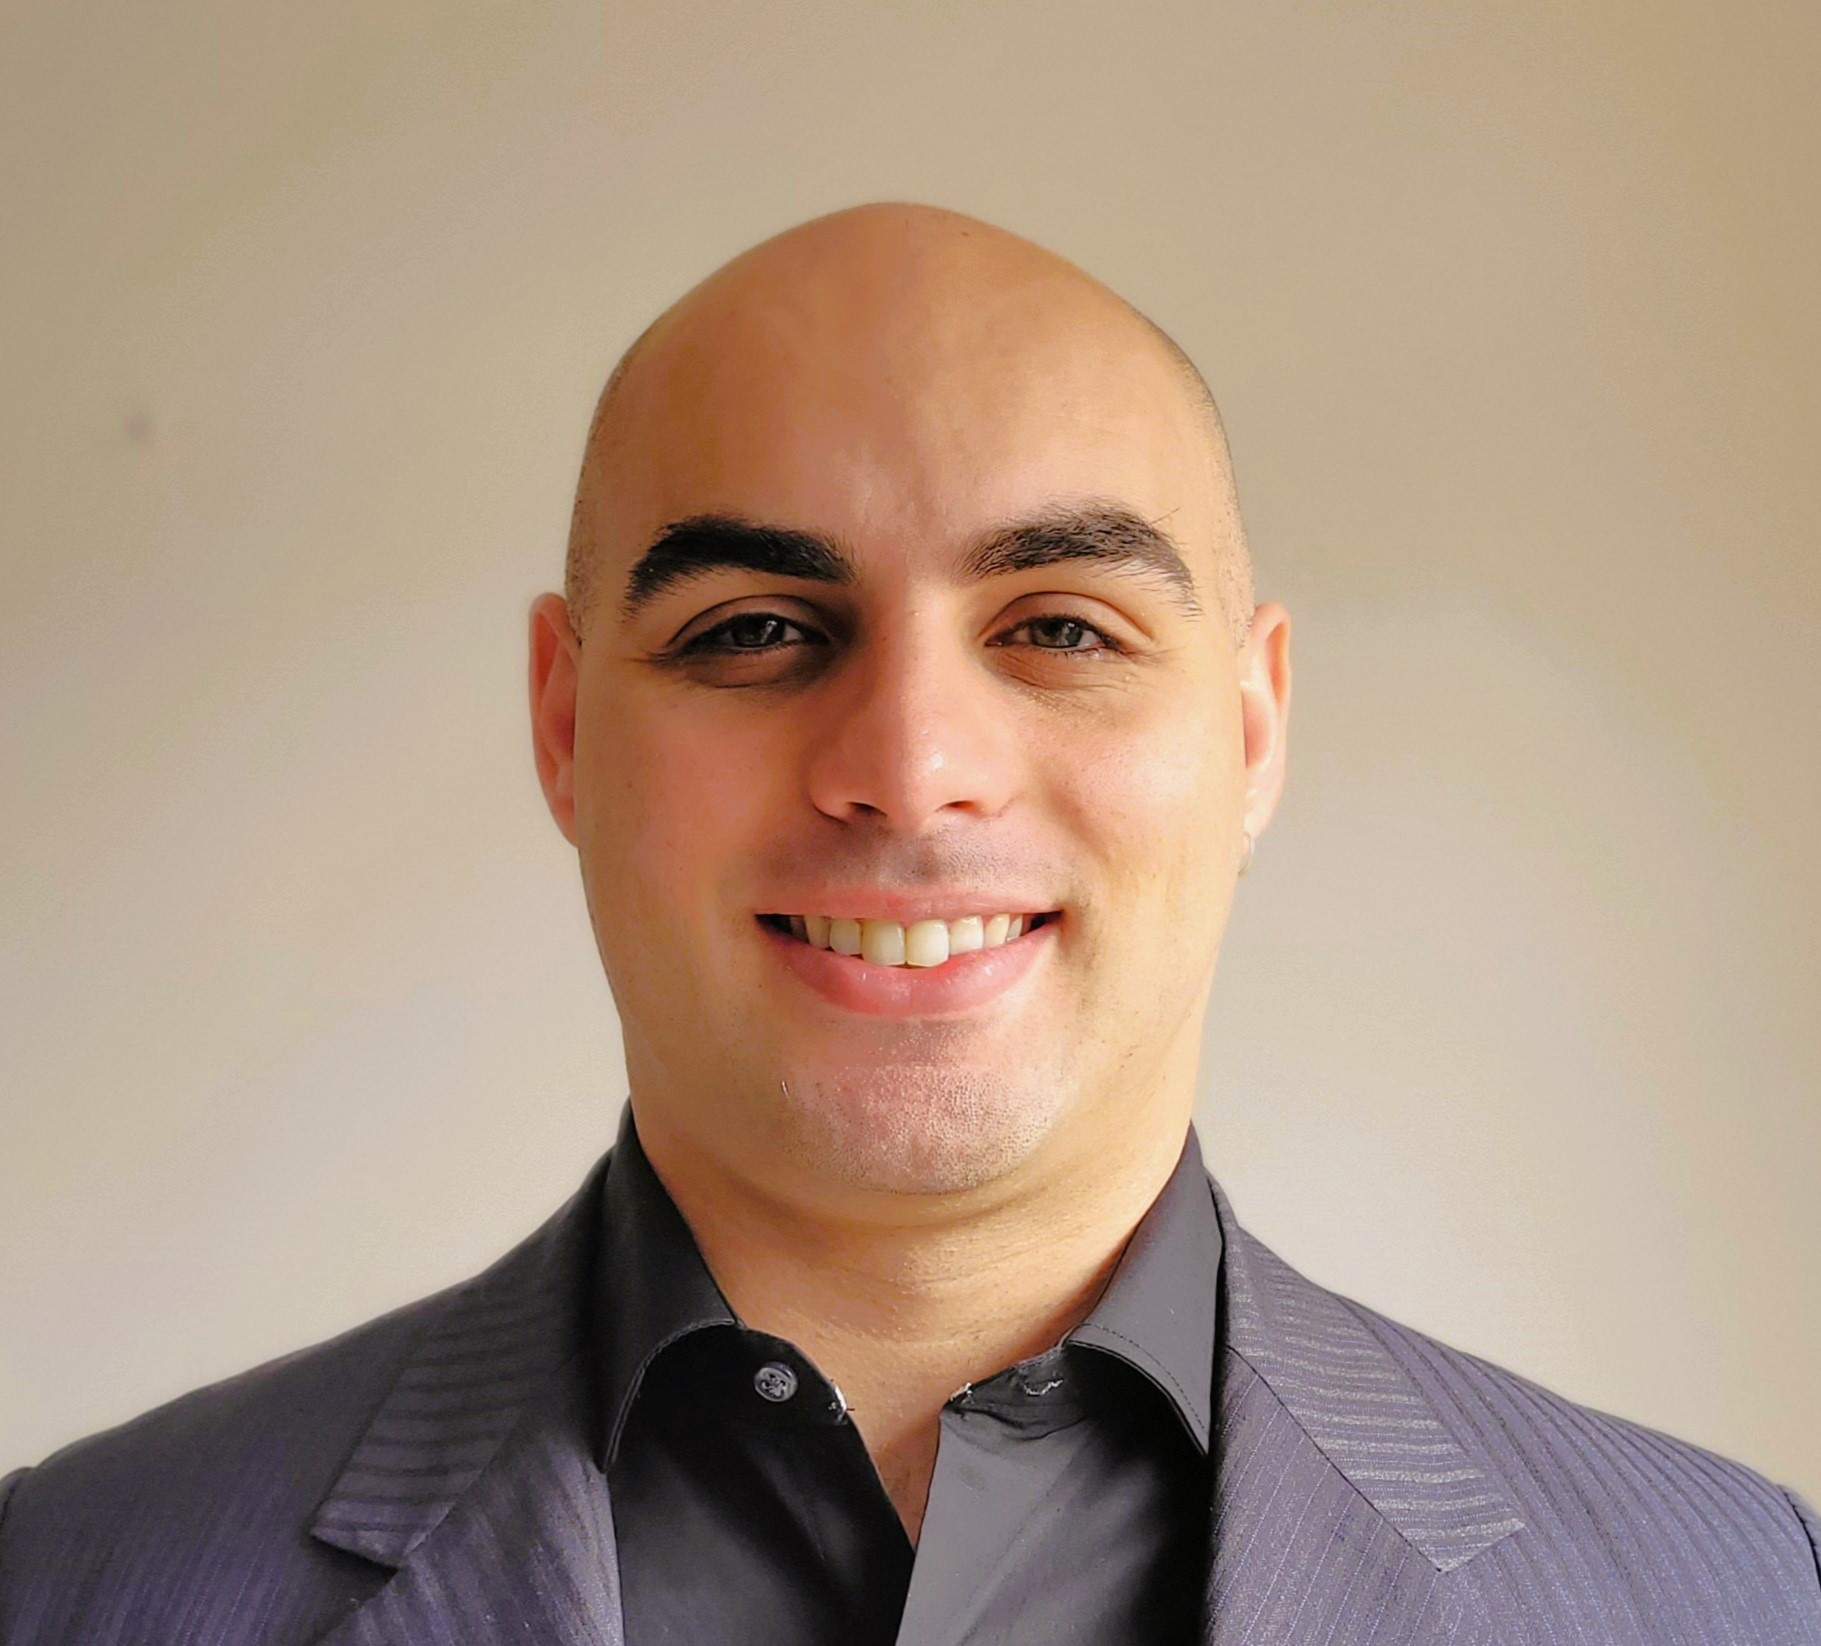
\includegraphics[width=\linewidth]{Foto.jpg}
    \end{figure}
    
    \cvsection{CONTACTO}

    \begin{tabular}{cl}
        {\Large\color{maincol}\faCalendar}                        & 01 de abril de 1992                                                       \\ [2pt]
        \multirow{2}{*}{{\Large\color{maincol}\faInfoCircle}}     & \href{https://goo.gl/maps/ciK9KomkCkJ7PdWt5}{Bahía Blanca} \href{https://goo.gl/maps/hbpY43DfhsFnmc8e6}{Buenos Aires,} \\ [2pt]
                                                                  & \href{https://goo.gl/maps/uPrySfuBds1QBUmq8}{Argentina}                   \\ [2pt]
        {\Large\color{maincol}\faAt}                              & \href{mailto:juanmcarini@gmail.com}{juanmcarini@gmail.com}                \\ [2pt]
        {\Large\color{maincol}\faPhone}                           & \href{tel:+5492914143811}{+54 (0291) 414 3811}                            \\ [2pt]
        {\Large\color{maincol}\faGithub}                          & \href{https://github.com/JuanMCarini}{JuanMCarini}                        \\ [2pt]
        {\Large\color{maincol}\faLinkedinSquare}                  & \href{https://www.linkedin.com/in/juanmcarini}{juanmcarini}
    \end{tabular}

    \cvsection{IDIOMAS}

    \begin{tabular}{ll}
        \textbf{Español:} & nativo \\ [2pt]
        \textbf{Ingles:}  & básico profesional.
    \end{tabular}

    \cvsection{HABILIDADES}

    \cvskill{SQL}      {0.3} 
    \cvskill{Python}   {0.4}
    \cvskill{Power BI} {0.5}
    \cvskill{Excel}    {0.8}
    \cvskill{\LaTeX}    {0.8}

\end{leftcolumn}

\begin{rightcolumn}
%===============================================================================================%
%   CABECERA
%===============================================================================================%
\fcolorbox{white}{darkcol}{\begin{minipage}[c][3cm][c]{0.99\mpwidth}
	\begin{center}
		\HUGE{ \textbf{ \textcolor{white}{ \uppercase{JUAN MARTÍN CARINI} } } } \\[-50pt]
		\textcolor{white}{ \rule{0.1\textwidth}{1.25pt} } \\[4pt]
		\large{\textcolor{white} {Lic.\@ en Matemática \& Científico de Datos}}
	\end{center}
\end{minipage}}
\vspace{6pt}

\cvsection{EDUCACIÓN}

    \itemedu{Data Science}
    {Marzo 2022 a la actualidad}{Coderhouse}
    \itemedu{\href{https://1drv.ms/b/s!Anr_tvZIYrhwgel_E2d7lqyOWQMaaQ}
            {Licenciatura en Matemática}}
            {Marzo 2010 a agosto de 2022}{Universidad Nacional del Sur}
    \vspace{-6pt}
    \hspace{0.2cm}\textit{\small\textbf{Materias Optativas:}}
        \begin{itemize}
            \footnotesize
            \item \href{https://1drv.ms/b/s!Anr_tvZIYrhwg-Q3BLmxwlzX5PWIFQ}{Principios de Computación I},
            \item \href{https://1drv.ms/b/s!Anr_tvZIYrhwg-Q45aG0UgNb-R70FA?e=44lo7C}{Introducción a los procesos estocásticos}.
        \end{itemize} 

    \itemedu{\href{https://www.coderhouse.com/certificados/620447e524e5820051a7aa74}
            {Data Analytics}}
            {Noviembre 2021 a febrero de 2022}{Coderhouse}

\cvsection{Cursos y Congresos}

    \itemedu{\href{https://1drv.ms/b/s!Anr_tvZIYrhwg-Q-or-wyygtVrYUuA?e=kgWNnG}
            {Curso de Python Intermedio}}
            {Agosto 2022}{Platzi}
    \itemedu{\href{https://1drv.ms/b/s!Anr_tvZIYrhwg8E-4q6mPHI1jq7ZLA?e=p6oXwW}
            {Curso Profesional de Git y GitHuB}}
            {Agosto 2022}{Platzi}
    \itemedu{\href{https://1drv.ms/b/s!Anr_tvZIYrhwgc9MosO5ebGk9rRf-w}
            {Reunión Anual de la UMA}}
            {Septiembre 2013}{Universidad Nacional de Rosario} 
    \itemedu{\href{https://1drv.ms/b/s!Anr_tvZIYrhwgc9GYBGAGbHQCQqjzQ}
            {XII Congreso Dr.\@ Antonio Monteiro}}
            {Mayo 2013}{Universidad Nacional del Sur}
    \itemedu{\href{https://1drv.ms/u/s!Anr_tvZIYrhwgc8YJ8r2Zmf6BP7aYg?e=ayx34k}
            {Introducción a Matlab}}
            {Noviembre 2012}{Dictado por la Mg.\@ Flavia Buffo en la Universidad Nacional del Sur}
    \itemedu{\href{https://1drv.ms/u/s!Anr_tvZIYrhwgc8af6-T-A7NeXaSlw}
            {Reunión Anual de Unión Matemática Argentina}}
            {Agosto 2012}{Universidad Nacional de Cordoba}
    \itemedu{\href{https://1drv.ms/u/s!Anr_tvZIYrhwgc8dRt9t2V22iKrg2g?e=do4ZLA}
            {XI Congreso Dr.\@ Antonio Monteiro}}
            {Mayo 2011}{Universidad Nacional del Sur} 
    \itemedu{\href{https://1drv.ms/u/s!Anr_tvZIYrhwgc8ZvQ58VgOIVIDOTA}
            {\LaTeX}}
            {Junio 2012}{Dictado por el Dr.\@ Marcelo Falappa en la Universidad Nacional del Sur}
    \itemedu{\href{https://1drv.ms/u/s!Anr_tvZIYrhwgc8dRt9t2V22iKrg2g}
            {XI Congreso Dr.\@ Antonio Monteiro}}
            {Mayo 2011}{Universidad Nacional del Sur}

\cvsection{Experiencia Laboral}

    \itememplo{Veterinaria El Destete}
    {Enero 2021 a febrero de 2022}
    {Encargado}
    {Atención de clientes}
    {Encargado del stock}
    {Actualización de precios en Marketplace (Facebook) y en la plataforma eCommerce}
    {Responsable de entradas y salidas en caja y cierre diario de la misma}

    \itememplo{Zammá Pasteleria \& Deco}
    {Febrero 2012 a agosto de 2020}
    {Vendedor}
    {Asesoramiento a los clientes}
    {Monitoreo de calidad y seguimiento de recepción de productos}
    {}{}

    \itememplo{Universidad Nacional del Sur}
    {Marzo 2012 a junio de 2019}
    {Ayudante alumno B}
    {Encargado de resolver dudas a los alumnos}
    {Corrección de exámenes parciales}
    {Ayudante en las asignaturas: Elementos de Algebra y Geometría, Algebra y Geometría y Calculo II, siendo parte del equipo docente.}
    {}


\end{rightcolumn}

\end{paracol}

\end{document}